\chapter{The Algorithm}

\section{Basis}

Our reconstruction uses the $\chi^2$ metric to determine which ordering of hits is best. Each triple represents one term in the sum of equation \ref{eq:chi2}. Since better orderings of hits produce more similar $\eta$ values, the ordering with the lowest value of $\chi^2$ is the most probable one. Therefore, we must try each possible ordering of hits in order to find the one that is best - a very computationally complex calculation. If there are $N$ hits in a photon event, there are $N!$ possible orderings of those hits, and we must recalculate the eta value for each hit in each ordering, adding an additional factor of $N$, to give us a total run-time of $O(N*N!)$ for each photon. There are several heuristic improvements we can make to this algorithm to shorten the average-case run-time, but we start with a basic iterative and sequential approach for simplicity's sake. The full pseudo-code can be found in Appendix \ref{app:code}.

\section{Performance improvement}
Though it is difficult to improve the worst-case time complexity of our algorithm, it is possible to make several changes that decrease the average run-time per photon. The most important of these changes is the switch from an iterative approach to a tree search, and the use of parallelism.

\subsection{Tree search}
The first and perhaps most important performance improvement we make is to change the structure of our program from an iterative approach - testing each sequence individually, one after another - to a recursive tree search. Each photon has its own tree, which refers to a type of data structure in computer science, containing 'nodes' of information - in our case, possible paths of the photon. Each parent node has a series of child nodes (excluding those at the end of the sequence), and to search the tree we simply have to choose a path through it, keeping track of the $\chi^2$ value as we go. Once we have searched each path we consider possible, we assume the path with the lowest $\chi^2$ value is the correct one and return its first two hits.  The first two hits are then all we need to estimate the scattering angle of the initial photon.

In our program, the nodes of our search tree each contain a Hit (a location and energy deposit) and a $\chi^2$ value for that point in the sequence. As we cannot start calculating the $\chi^2$ value without at least one triple, we first take each possible pair of hits and run them through our recursive search algorithm, keeping a running tally of the $\chi^2$ value and updating it for each child node we process. Theoretically, we would still have to process every possible sequence before reaching a conclusion about the minimum $\chi^2$ value, but, as discussed in the next section, there are ways to decrease the average-case runtime. The real performance improvement of the tree comes from the recursive approach. In our iterative approach, we recalculated $\chi^2$ for each node, including those which had the same parent node (giving them the same $\chi^2$ value). In the recursive approach, we cut down on these repeat calculations by carrying the $\chi^2$ value through each sequence and only adding onto it when we process a new node. 

- provide pseudocode

\subsection{Pre-calculation of $\eta$ values}
Another performance improvement comes from pre-calculating the spatial angles for each triple. In the sequential/iterative algorithm, we calculate $\eta$ for each triple in each sequence, but unlike $\eta'$, the spatial angle does not change based on the previous ordering of hits. As it is only based on the hits in its given triple, we can calculate $\eta$ once for each possible triple before we start the tree search and fetch the values when they come up in order to reduce our run-time per photon.

\subsection{$\chi^2$ and $\eta$ cutoffs}

During our tree search, we can 'prune' some sub-trees by filtering out some possible sequences before we process the final hit. Theoretically, we could still end up having to search the whole tree for the correct path depending on which values we use to prune, but generally these methods will improve our run-time in the average case. We prune a sub-tree if:
\begin{enumerate}
    \item The $\chi^2$ value is already greater than the running minimum.
    \item The energetically reconstructed cos(angle), $\eta'$, is greater than 1 by some amount.
    \item The $\chi^2$ value exceeds what we would expect for a given p-value.
\end{enumerate}
The p-value of an ordering is related to the probability of getting some $\chi^2$ value with the number of degrees of freedom as the number of hits we have added to the value so far. We use a look-up table to find the estimated $\chi^2$ value, such as the one shown in figure \ref{fig:p-val}. For example, if we choose a p-value of 0.10, we will not accept any orderings that have less than a 10\% chance of being correct. So, from the table, we will cut off computation for $\chi^2$ values greater than 2.76 for one hit, 4.605 for two hits, 6.251 for three hits, etc.

\begin{figure}
    \centering
    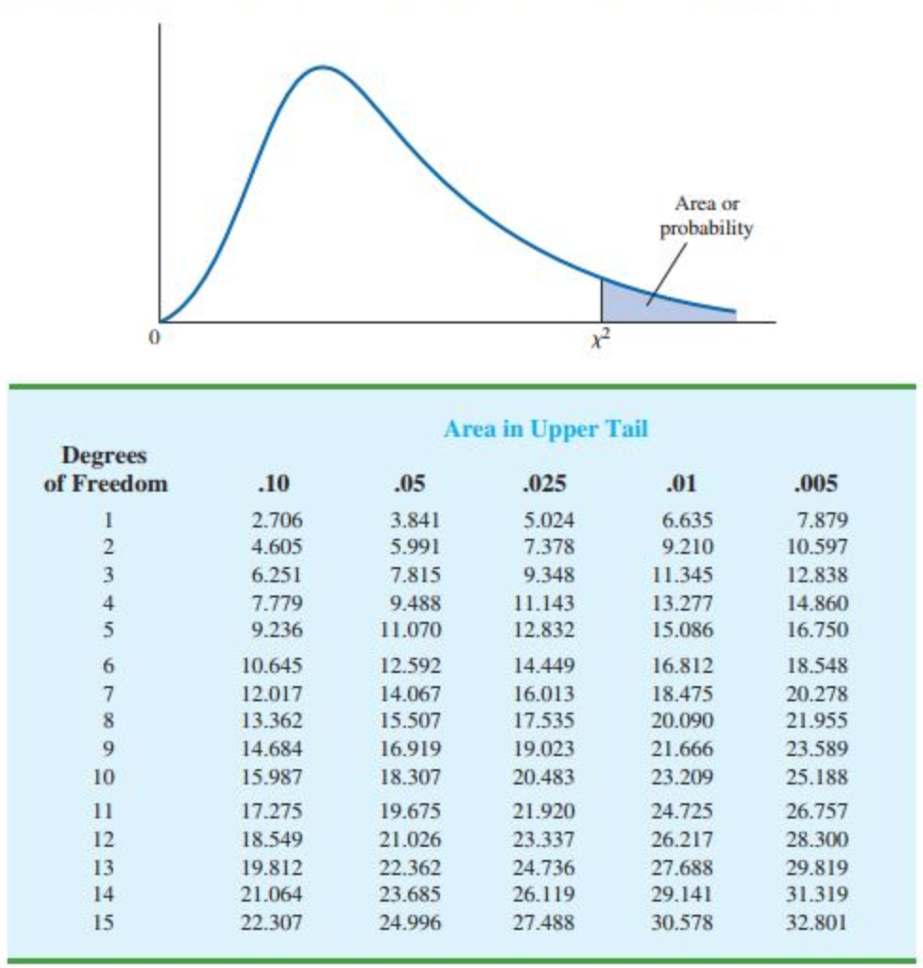
\includegraphics[width=0.5\textwidth]{chi2table.png}
    \caption{An example $\chi^2$ look-up table \cite{chitable}.}
    \label{fig:p-val}
\end{figure}

\section{Parallelism}
Our final performance improvement comes from parallelism - each photon's computation may be run in parallel with the others' to reduce the total running time of our algorithm. This means that if any given photon's computation takes longer than real-time there will not be a backlog of events to process, which would delay the localization of a gamma-ray burst or other transient. The easier photons to process, with fewer numbers of hits, will naturally complete first. This is perfect for our problem, as we expect there to be more photons with small numbers of hits than those with larger numbers of hits. If we need a quick reading of a GRB source, we can get a broader position first using these easier-to-calculate photons and allow the more complicated events to increase the accuracy of our estimate after the fact.

As our current level of parallelism was able to adequately meet our time constraints, we do not run any other part of our computation in parallel, but there are several different ways we could implement this depending on future time constraints. For longer computations, we could save time by running a certain number of sub-trees in parallel threads and finding the lowest $\chi^2$ afterward. We could also calculate some of the spatial angles in parallel, as these increase proportionally to $N^3$.

\section{Comparison}

The improvements we made to our algorithm made a significant difference in terms of overall performance. The sequential/iterative version of the algorithm could process only 1000 photons per second, while the tree search algorithm can process over 50,000 photons per second at its best performance.

\iffalse
\label{cpt:citation}

In the References section at the end of your thesis, list references cited
using the style recommended in \textit{The Chicago Manual of
Style}~\cite{ChicagoManual} or another style acceptable to your committee.
Insert parenthetical references where the reference material is referred to in
the text.  This chapter explains how to format references according to
\textit{The Chicago Manual of Style}.  If you use a different style, you should
obtain the appropriate style rules.  For example, most journals periodically
print instructions for authors that include reference style rules.

\section{Parenthetical References}

References should be cited at the position in the text where they are noted.
\textit{The Chicago Manual of Style}~\cite{ChicagoManual} recommends two
systems for citations.  You may use either of these systems or an alternative
system acceptable to your committee.

\subsection{Author-Date System}

In this system, the last name of the author and the year of
publication appear in parentheses following the quoted text.  If the
reference is alphabetized in the References section by its editor,
publisher, or organization, then the name it is alphabetized under is
used in place of the author.  Some examples follow:
\begin{itemize}
 \item Single author: (Smith 1993)
 \item Two authors: (Jones and Yang 1991)
 \item Three authors: (Jones, Smith, and Yang 1984)
 \item Four or more authors: (Johnson et al. 1994)
 \item Organization as author: (Association for Computing Machinery 1989)
 \item Two works referenced in one sentence: (Black 1994; Smith 1993)
\end{itemize}

\subsection{Numbered References}

In this system, the reference number appears in square brackets following the
quoted text.  This system is used throughout this document.

\section{Reference List}

References should be listed in alphabetical order by the last name of the first
author (or organization or publisher, if no author is given).  If the numbered
reference style is used, the reference list should obviously be numbered as
well.  Several example references are listed in this document's reference list.
Most of these references are taken from \textit{A Manual for Writers of Term
Papers, Theses, and Dissertations}~\cite{Turabian}.
\fi

%%% Local Variables: 
%%% mode: latex
%%% TeX-master: "thesis-main"
%%% End: 
